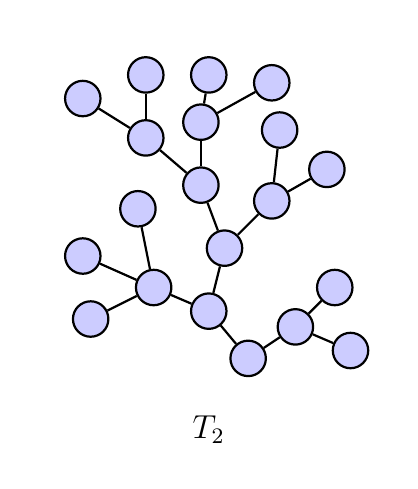
\begin{tikzpicture}[
  baseline=0pt,
  scale=1,
  vnode/.style={circle, draw=black, fill=blue!20, thick, inner sep=0pt, minimum size=4.5mm},
  edge/.style={thick, draw=black}
]
  \useasboundingbox (-2.3,-3.1) rectangle (2.3,2.4);

  % Reflejos verticales manteniendo los límites y=-1.8 y y=1.8
  \begin{scope}[yscale=-1]
    \node[vnode] (v1) at (0.5, 1.8) {};
    \node[vnode] (v2) at (0.0, 1.2) {};
    \node[vnode] (v3) at (1.1, 1.4) {};
    \node[vnode] (v4) at (1.8, 1.7) {};
    \node[vnode] (v5) at (1.6, 0.9) {};
    \node[vnode] (v6) at (-0.7, 0.9) {};
    \node[vnode] (v7) at (0.2, 0.4) {};
    \node[vnode] (v8) at (-1.5, 1.3) {};
    \node[vnode] (v9) at (-1.6, 0.5) {};
    \node[vnode] (v10) at (-0.9, -0.1) {};
    \node[vnode] (v11) at (0.8, -0.2) {};
    \node[vnode] (v12) at (-0.1, -0.4) {};
    \node[vnode] (v13) at (1.5, -0.6) {};
    \node[vnode] (v14) at (0.9, -1.1) {};
    \node[vnode] (v15) at (-0.8, -1.0) {};
    \node[vnode] (v16) at (-0.1, -1.2) {};
    \node[vnode] (v17) at (-1.6, -1.5) {};
    \node[vnode] (v18) at (-0.8, -1.8) {};
    \node[vnode] (v19) at (0.0, -1.8) {};
    \node[vnode] (v20) at (0.8, -1.7) {};

    % Aristas
    \draw[edge] (v1) -- (v2); \draw[edge] (v1) -- (v3);
    \draw[edge] (v3) -- (v4); \draw[edge] (v3) -- (v5);
    \draw[edge] (v2) -- (v6); \draw[edge] (v2) -- (v7);
    \draw[edge] (v6) -- (v8); \draw[edge] (v6) -- (v9); \draw[edge] (v6) -- (v10);
    \draw[edge] (v7) -- (v11); \draw[edge] (v7) -- (v12);
    \draw[edge] (v11) -- (v13); \draw[edge] (v11) -- (v14);
    \draw[edge] (v12) -- (v15); \draw[edge] (v12) -- (v16);
    \draw[edge] (v15) -- (v17); \draw[edge] (v15) -- (v18);
    \draw[edge] (v16) -- (v19); \draw[edge] (v16) -- (v20);
  \end{scope}

  % Etiqueta
  \node[font=\large] at (0,-2.7) {$T_2$};
\end{tikzpicture}
